\documentclass[conference]{IEEEtran}

\usepackage[utf8]{inputenc}
\usepackage[T1]{fontenc}
\usepackage[english]{babel}
\usepackage{array}
\usepackage[table]{xcolor}
\usepackage{makecell}
\usepackage{amsmath}
\usepackage{amssymb}
\usepackage{graphicx}
\usepackage{booktabs}
\usepackage{tabularx}
\usepackage{tikz}
\usetikzlibrary{arrows.meta, positioning}
\usepackage{placeins}
\usepackage{enumitem}
\usepackage[hyphens]{url}
\usepackage[colorlinks=true,allcolors=black]{hyperref}
\usepackage{soul} % \ul
\setuldepth{Berlin}

\newcommand{\cmark}{\textbf{X}} % symbol to mark cells
\newcommand\red[1]{{\textcolor{red}{#1}}}

\title{Native Vector-Symbolic Networks for Composing Independently Trained Models:\\
Architecture, Protocol and Empirical Validation}

\author{
\IEEEauthorblockA{Creative Experience: Transformative Project II\\
Bachelor’s in Computer Science -- PUCPR
\\[3ex]
Class 8B -- Team 11 \\
Bruno Betiatto, Mohamad Diab, Henrique Godoy, Lucca Magalhães, Gabriel Schneider \\
{\tt\small \{bruno.betiatto, mohamad.diab, henrique.godoy, lucca.magalhaes, gabriel.schneider\}@pucpr.edu.br}
}
}

\date{today}

\sloppy
\begin{document}

\maketitle

\begin{abstract}
We investigate a neural architecture that represents its own hidden state as a
vector-symbolic program: sparse, overlapping groups of units are pooled, bound
to role vectors, discretised against per-group codebooks and bundled into a
graded unary-plus-pairwise program. The aim is to compose independently trained
networks algebraically rather than by retraining. This paper validates the
representation such a composition would depend on. We define a single
cross-domain protocol with a fixed architecture, declared ablation axes and
fold-paired statistics, and apply it to MNIST, Fashion-MNIST, BloodMNIST and
DermaMNIST. One configuration transfers across all four without retuning; the
discrete bottleneck costs essentially nothing in accuracy and about $0.008$
macro AUC; and the groups, trained only to classify, converge on redundant
codes. An inter-group mutual-information penalty roughly doubles the
compositional gain at no accuracy cost, while degrading hypervector recovery,
the property the composition mechanism itself requires.
\end{abstract}

\section{Project Description}
\label{sec:intro}

Vector symbolic architectures (VSAs), otherwise known as hyperdimensional computing (HDC), are a cognitive-algebraic framework for representing and manipulating symbol-like structures using algebraic operations (binding, bundling, permutation) on very high-dimensional vectors, or ``hypervectors''~\cite{kanerva2009hyperdimensional,kleyko2022survey}.

Zhang, Jiang, and Quan~\cite{zhang2025formalisms} have recently argued that the choice between knowledge representation methodologies, a longstanding debate in AI and AGI, does not actually buy anything in expressive power: much the contrary, all ``universal'' knowledge representation formalisms are recursively isomorphic to one another, so that for any knowledge operator in one formalism (e.g., gradient descent) there exists an operationally equivalent operator in another. Thus, hyperdimensional computing has experienced a recent resurgence as a potential bridge between connectionist and symbolic AI (an approach known as neurosymbolic AI), due to the shortcomings of each alone. Results have been mostly positive, with neural networks supported by hypervectors demonstrating greater systematic and compositional reasoning capabilities not typically observed in purely neural systems. Hersche et al.'s~\cite{hersche2023nvsa} neuro-vector-symbolic architecture, for instance, used hypervectors as a shared representational code between neural and symbolic components to set a new accuracy record on Raven's Progressive Matrice.

Optimism aside, the integration between the inherently procedural, continuous connectionism and the declarative, discrete symbolism has been notoriously difficult, with the majority of proposed systems either demonstrating only superficial integration or collapsing into one paradigm. Some authors refer to this as the differentiability gap, and the problem spills over to Harnad's~\cite{harnad1990symbol} famous exposition of the symbol grounding problem. Furthermore, representing symbols as vectors in extremely high-dimensional spaces currently presents several practical implementation difficulties on standard, modern hardware.

But the actual reason VSAs first appeared intriguing to AI has been largely underexplored. That is, their potential as a translator between specialized areas of the brain, or between separately-trained modules more generally. Recent work by Sutor et al.~\cite{sutor2022gluing} has explored integrating separately trained neural networks through a mechanism they call HD-Glue, which encodes each network's final-layer output signals as a hypervector; these per-network hypervectors are then bundled together into a single consensus hypervector that the fused networks jointly ``vote'' on to produce a prediction.

We aim to take this further, and propose to investigate a new architecture that natively thinks in hypervectors; we will create hidden, cross-layer neuron aggregations, which will be projected to hypervectors. Backpropagation will be used to train the network's hypervectors, and vice-versa. Then, after training, we will pool these hypervectors, bind them into a common network hypervector, and eventually connect two independently trained models using an algebraic glue mechanism of our own. With this, we aim a twofold contribution: a proposed native neurosymbolic architecture in the Fodor and Pylyshyn~\cite{fodor1988connectionism} sense, and a way forward to compose such architectures as an alternative to pure, uniform scaling.


\begin{figure*}[t]
\centering
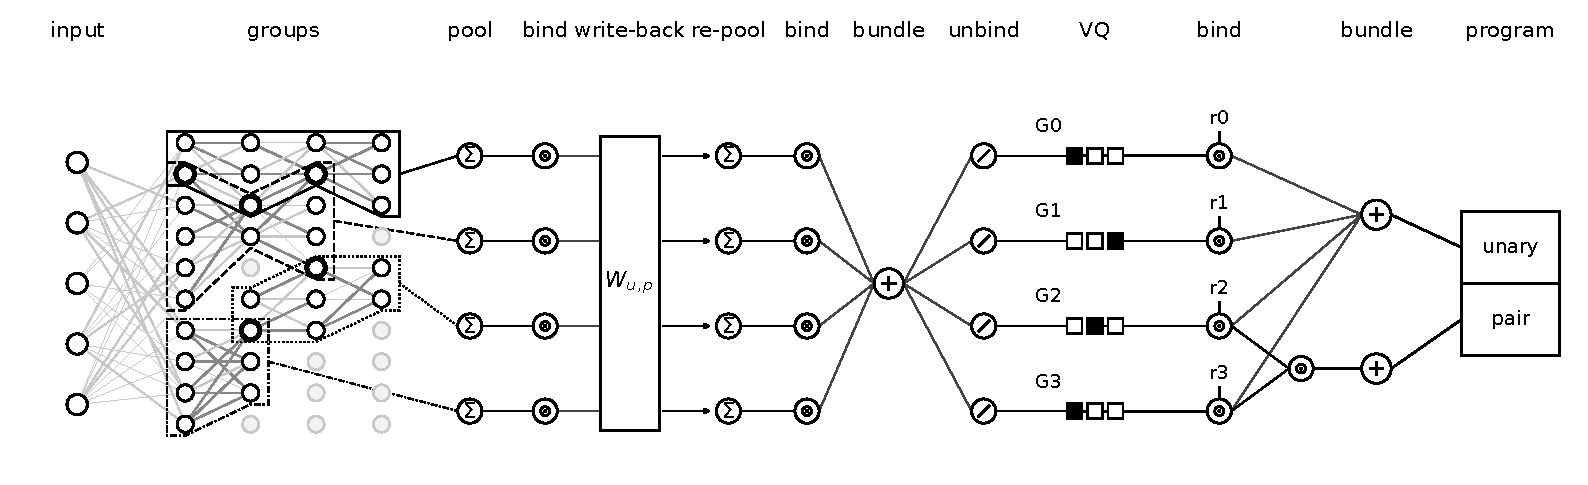
\includegraphics[width=0.92\textwidth]{figs/architecture.pdf}
\caption{\texttt{SparseJointCore} pipeline: the input is projected onto sparse, overlapping \emph{groups}; each group is pooled and bound to a role vector, written back onto its shared units, and re-pooled; the resulting values are bound and bundled into a unary code, then unbound per group and quantized against each group's codebook ($G_0$--$G_3$); the quantized values are re-bound to their roles and bundled twice, once for the unary program and once for the pairwise program (connected-group products), forming the final [unary; pair] program.}
\label{fig:method}
\end{figure*}

Figure~\ref{fig:method} summarises the core as implemented. The target
application is the MOVi benchmark from Kubric~\cite{greff2022kubric}, synthetic
video scenes with rigid-body physics, around which three specialists are
defined: a vision specialist (CNN+GRU), a physics specialist (MLP+GRU with a
code-dynamics model) and an outcome decoder. Composing two such specialists
requires the Glue of Figure~\ref{fig:glue}, which decomposes the pairwise joint
code distribution of connected groups into an ANOVA-style interaction term and
solves, per connected component of the scaffold, for the permutation that best
matches those terms between two networks, without paired labels.

That composition step is not what this paper validates. Random, uncorrelated
data yields a near-zero alignment objective by construction, so a meaningful
Glue test needs real paired codes, which are not yet available. What we can
establish now, and what Sections~\ref{sec:protocol} and~\ref{sec:results} do
establish, is whether the representation the Glue would have to operate on is
sound: whether the same core transfers across domains, what the discrete
bottleneck costs, and whether the groups carry complementary information at all
or merely duplicate each other. The last of these turns out to require an
explicit intervention, and that intervention has a measurable price.

\begin{figure}[t]
\centering
\begin{minipage}{0.4\linewidth}
\centering
\resizebox{\linewidth}{!}{%
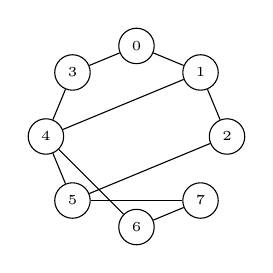
\begin{tikzpicture}[every node/.style={circle, draw, minimum size=4.5mm, font=\tiny, inner sep=0pt}]
\foreach \i/\ang in {0/90,1/45,2/0,3/135,4/180,5/225,6/270,7/315}{
  \node (n\i) at (\ang:1.15) {\i};
}
\draw (n0)--(n1); \draw (n0)--(n3); \draw (n1)--(n2); \draw (n1)--(n4);
\draw (n2)--(n5); \draw (n3)--(n4); \draw (n4)--(n5); \draw (n4)--(n6);
\draw (n5)--(n7); \draw (n6)--(n7);
\end{tikzpicture}%
}
\centerline{\scriptsize (a) scaffold graph ($G{=}8$)}
\end{minipage}%
\hfill
\begin{minipage}{0.52\linewidth}
\centering
\resizebox{\linewidth}{!}{%
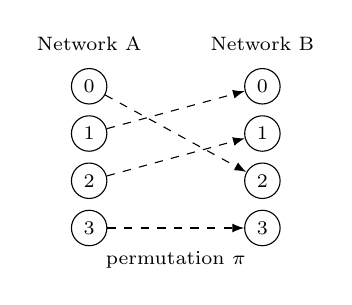
\begin{tikzpicture}[every node/.style={font=\scriptsize}]
\tikzset{grp/.style={circle, draw, minimum size=4.5mm, inner sep=0pt}}
\foreach \i in {0,...,3}{
  \node[grp] (a\i) at (0,-\i*0.6) {\i};
  \node[grp] (b\i) at (2.2,-\i*0.6) {\i};
}
\node[above=1mm of a0] {Network A};
\node[above=1mm of b0] {Network B};
\draw[-{Latex[length=1.5mm]}, dashed] (a0) -- (b2);
\draw[-{Latex[length=1.5mm]}, dashed] (a1) -- (b0);
\draw[-{Latex[length=1.5mm]}, dashed] (a2) -- (b1);
\draw[-{Latex[length=1.5mm]}, dashed] (a3) -- (b3);
\node at (1.1,-2.2) {\scriptsize permutation $\pi$};
\end{tikzpicture}%
}
\centerline{\scriptsize (b) Glue concept}
\end{minipage}
\caption{(a) The scaffold graph actually used for $G=8$ groups (\texttt{make\_rigid\_scaffold}): an edge means the two groups share a physical unit in some layer, so pairwise messages and Glue alignment only ever cross these edges. (b) Glue concept: \texttt{fit\_sj\_glue} finds the per-component code permutation $\pi$ that aligns two independently trained networks' groups, using only the (unpaired) statistics of their connected-group code distributions.}
\label{fig:glue}
\end{figure}



% =====================================================================
% Seção de metodologia e validação — artigo sparse-joint networks
%
% Mantida no repositório, ao lado do código que produz os números:
%   validation.py  gera results/validation/*.json
%   report.py      gera results/validation/paper/{tables,figuras}
%
% Para usar no artigo, copie as tabelas e figuras geradas para figs/ e
% faça % =====================================================================
% Seção de metodologia e validação — artigo sparse-joint networks
%
% Mantida no repositório, ao lado do código que produz os números:
%   validation.py  gera results/validation/*.json
%   report.py      gera results/validation/paper/{tables,figuras}
%
% Para usar no artigo, copie as tabelas e figuras geradas para figs/ e
% faça % =====================================================================
% Seção de metodologia e validação — artigo sparse-joint networks
%
% Mantida no repositório, ao lado do código que produz os números:
%   validation.py  gera results/validation/*.json
%   report.py      gera results/validation/paper/{tables,figuras}
%
% Para usar no artigo, copie as tabelas e figuras geradas para figs/ e
% faça \input{methodology} depois da seção de trabalhos relacionados.
%
% Requer no preâmbulo (já presentes no template): graphicx, booktabs,
% tikz (arrows.meta, positioning), amsmath.
% =====================================================================

\section{The Sparse-Joint Core}
\label{sec:architecture}

A sparse-joint network replaces the dense bottleneck of a conventional encoder
with a \emph{graded program}: a representation that is simultaneously discrete,
as a tuple of per-group symbols, and continuous, as a hypervector that the
network can differentiate through. This section states the construction
precisely; Section~\ref{sec:protocol} describes how we test it.

\subsection{Groups and the scaffold}

Let $U$ be the number of hidden units per layer, $L$ the number of layers and
$G$ the number of \emph{groups}. A group is a sparse population of units
distributed across layers, fixed before training by a binary mask
$M \in \{0,1\}^{L \times G \times U}$, where $M_{l,g,u}=1$ means that group $g$
owns unit $u$ in layer $l$. We call $M$ the \emph{scaffold}.

Two groups are adjacent when they physically share a unit:
\begin{equation}
  (i,j) \in E \iff \exists\, l,u : M_{l,i,u} = M_{l,j,u} = 1 .
  \label{eq:edges}
\end{equation}
The edge set $E$ is therefore not a hyperparameter chosen alongside the
architecture; it is a \emph{consequence} of the scaffold, readable from the
weights themselves. This is what later allows $E$ to act as a compatibility
certificate between two independently trained networks: two networks with
isomorphic scaffolds expose the same relational skeleton, even though neither
has seen the other's data. Figure~\ref{fig:glue}(a) shows the graph used
throughout this work, for $G=8$.

Unit-to-unit transitions are routed through the scaffold: a connection between
units $u$ and $u'$ exists only if some group contains both. A group therefore
cannot read an arbitrary part of the hidden state, which is what makes the
sparsity structural rather than merely a regulariser.

\subsection{From activations to a program}

Write $h^{(l)} \in \mathbb{R}^{U \times W}$ for the hidden state at layer $l$,
each unit carrying a width-$W$ vector, with
$h^{(0)} = \mathrm{GELU}(W_{\text{in}}\, \phi(x))$ for an encoder $\phi$. Each
group pools the units it owns, across all layers:
\begin{equation}
  f_g = \frac{1}{L}\sum_{l=1}^{L}
        \frac{\sum_{u} M_{l,g,u}\, h^{(l)}_u}{\sum_{u} M_{l,g,u}},
  \qquad
  v_g = \frac{W_{\text{val}} f_g}{\lVert W_{\text{val}} f_g \rVert}.
  \label{eq:pool}
\end{equation}

Each group owns a fixed bipolar \emph{role} vector $r_g \in \{-1,+1\}^{D}$,
drawn once at initialisation. Binding is the Hadamard product, the standard
multiply-add vector-symbolic algebra: $r_g \odot v_g$ binds the group's value to
its identity, and because $r_g \odot r_g = \mathbf{1}$, binding again by the
same role unbinds it. Unary messages are written back to every unit the group
owns, and pairwise messages $r_i v_i \odot r_j v_j$ only to the units that $i$
and $j$ physically share, so interaction is confined to $E$ by construction.
The stack is then re-pooled, giving refined values $v'_g$.

The refined values are superposed into a single hypervector, and each group is
recovered from the superposition by unbinding with its own role:
\begin{equation}
  b = \frac{1}{\sqrt{G}}\sum_{g=1}^{G} r_g \odot v'_g,
  \qquad
  \tilde{v}_g = \sqrt{G}\, \bigl( b \odot r_g \bigr).
  \label{eq:bundle}
\end{equation}
Recovery is approximate: the other $G-1$ terms survive as noise whose magnitude
falls with $D$. We measure this directly (Section~\ref{sec:protocol},
\emph{VSA recovery}) rather than assuming it, because every downstream claim
about reading codes back out depends on it.

\subsection{Discretisation}

Each group owns a codebook $C_g \in \mathbb{R}^{K_g \times D}$ with its own
alphabet size $K_g$, so groups need not share a vocabulary. Cleanup is a cosine
lookup against that codebook,
\begin{equation}
  \ell_{g,c} = \frac{1}{\tau}
  \left\langle \frac{\tilde{v}_g}{\lVert \tilde{v}_g \rVert},
               \frac{C_{g,c}}{\lVert C_{g,c} \rVert} \right\rangle
  + m_{g,c},
  \label{eq:cleanup}
\end{equation}
where $m_{g,c} = -\infty$ for $c \geq K_g$ masks out fillers outside the group's
alphabet. The discrete code is $z_g = \arg\max_c \ell_{g,c}$, and gradients pass
through a straight-through estimator~\cite{bengio2013estimating,oord2017neural}, so the forward pass is exactly discrete
while the backward pass stays differentiable.

The exported \emph{program} is graded, concatenating a unary and a pairwise
bundle:
\begin{equation}
  \begin{aligned}
    P(x) &= \bigl[\, p_{\text{unary}} \;;\; p_{\text{pair}} \,\bigr],\\
    p_{\text{unary}} &= \tfrac{1}{\sqrt{G}}\textstyle\sum\nolimits_g r_g \odot \hat{v}_g,\\
    p_{\text{pair}} &= \tfrac{1}{\sqrt{|E|}}\textstyle\sum\nolimits_{(i,j) \in E}
       \hat{h}_i \odot \hat{h}_j,
  \end{aligned}
  \label{eq:program}
\end{equation}
where $\hat{h}_g = r_g \odot \hat{v}_g$ is the bound contribution of group $g$,
and $\hat{v}_g$ the quantised value of group $g$. The first term says what each
part is; the second says which parts co-occur, and only along scaffold edges.
Figure~\ref{fig:method} traces the whole path.

\subsection{Redundancy between groups}
\label{sec:penalty}

Nothing in Equations~\ref{eq:pool} to~\ref{eq:program} forces groups to encode
\emph{different} things. Trained only to classify, every group independently
converges on the label: the codes become near-copies of one another, and the
pairwise term of Equation~\ref{eq:program} carries nothing the unary term does
not already carry. We confirm this empirically in Section~\ref{sec:results}.

We therefore add a penalty on the mutual information between the soft code
distributions of every pair of groups. Writing $p_g \in \Delta^{K_g}$ for the
posterior of group $g$ on a batch, and $\hat{p}_{ij}$ for the empirical joint,
\begin{equation}
  \mathcal{L}_{\text{red}} =
  \frac{1}{G(G-1)} \sum_{i \neq j}
  \sum_{c,c'} \hat{p}_{ij}(c,c')
  \log \frac{\hat{p}_{ij}(c,c')}{\hat{p}_i(c)\,\hat{p}_j(c')},
  \label{eq:redundancy}
\end{equation}
added to the task loss with weight $\lambda$. Minimising it pushes the groups
towards statistically independent codes. The full objective is
$\mathcal{L} = \mathcal{L}_{\text{task}} + \mathcal{L}_{\text{VQ}}
+ \mathcal{L}_{\text{support}} + \lambda \mathcal{L}_{\text{red}}$.

% =====================================================================

\section{Experimental Protocol}
\label{sec:protocol}

The claims this architecture makes are about generality and about structure,
not only about accuracy, so the protocol has to be comparable across domains
and has to measure structure explicitly.

\subsection{Architecture and ablation axes}

Every result reported here uses the same core configuration: $G=8$ groups,
alphabet $K_g=16$, $U=128$ units, $L=3$ layers, $D=256$, unit width $8$, trained
for 120 epochs with AdamW at a learning rate of $2\times10^{-3}$ and batch
size 1024.\footnote{The epoch count is set so that the number of optimiser steps
matches that of the smaller-batch configuration it replaced, making the two
training budgets comparable.} Only three axes vary, and each is named in the
configuration:

\begin{itemize}[leftmargin=*, itemsep=1pt, topsep=2pt]
  \item \textbf{encoder}, a single dense layer over flattened pixels, or a
        small CNN, both mapping into the same $\phi$ dimensionality;
  \item \textbf{core}, the sparse-joint core or a dense bottleneck of
        identical output dimensionality, used as a control;
  \item \textbf{$\lambda$}, the weight of the redundancy penalty of
        Equation~\ref{eq:redundancy}.
\end{itemize}

This matters for comparability. In an earlier state of this
work the image-classification experiments and the medical-imaging experiments
ran under different core configurations ($L=2, U=32, D=64$ against
$L=3, U=128, D=256$), which makes any cross-domain comparison between them
meaningless. Fixing the architecture is what licenses the generality claim in
Section~\ref{sec:results}.

\subsection{Validation}

We use stratified $k$-fold cross-validation with $k=5$ rather than the official
benchmark splits, pooling all official partitions first. Three consequences
follow, and all three are deliberate:

\begin{enumerate}[leftmargin=*, itemsep=1pt, topsep=2pt]
  \item every sample is evaluated exactly once, which matters on the smaller
        medical datasets where a single test split is noisy;
  \item the fold partitions are generated from a fixed seed and are
        \emph{identical across configurations}, so a comparison between two
        configurations is paired fold by fold;
  \item standardisation statistics are computed on the training fold only.
\end{enumerate}

Datasets are stratified-subsampled to a common ceiling of 17{,}000 samples, so
that MNIST does not receive four times the training budget of BloodMNIST. Where
a comparison is drawn between configurations, we report the paired difference
per fold, Cohen's $d$, and a Wilcoxon signed-rank $p$-value. With five folds
that test has little power; the effect size is the primary reading and the
$p$-value is reported for completeness rather than as a decision rule.

\begin{figure}[!t]
\centering
\resizebox{0.99\linewidth}{!}{%
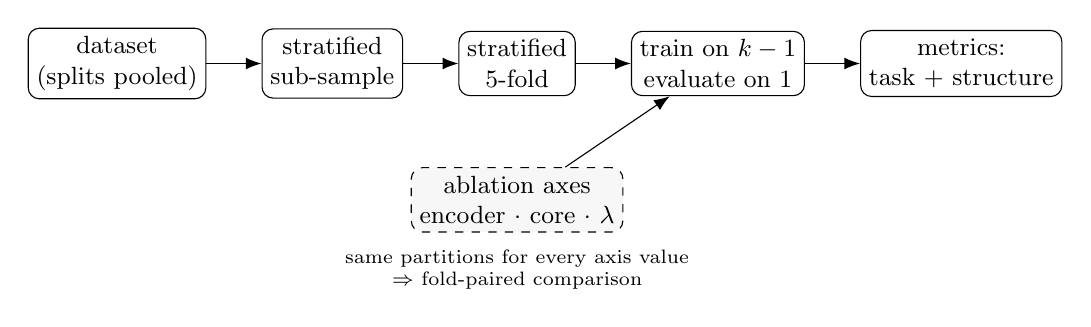
\begin{tikzpicture}[font=\small, node distance=3mm]
\tikzset{
  box/.style={draw, rounded corners, align=center, minimum height=8mm, inner sep=3pt},
  ax/.style={draw, dashed, rounded corners, align=center, inner sep=3pt, fill=black!3},
}
\node[box] (data) {dataset\\(splits pooled)};
\node[box, right=7mm of data] (cap) {stratified\\sub-sample};
\node[box, right=7mm of cap] (fold) {stratified\\5-fold};
\node[ax, below=9mm of fold] (axes) {ablation axes\\encoder $\cdot$ core $\cdot$ $\lambda$};
\node[box, right=7mm of fold] (train) {train on $k-1$\\evaluate on $1$};
\node[box, right=7mm of train] (met) {metrics:\\task $+$ structure};

\draw[-{Latex[length=2mm]}] (data) -- (cap);
\draw[-{Latex[length=2mm]}] (cap) -- (fold);
\draw[-{Latex[length=2mm]}] (fold) -- (train);
\draw[-{Latex[length=2mm]}] (train) -- (met);
\draw[-{Latex[length=2mm]}] (axes) -- (train);
\node[below=1mm of axes, font=\scriptsize, align=center]
  {same partitions for every axis value\\$\Rightarrow$ fold-paired comparison};
\end{tikzpicture}%
}
\caption{The protocol. Fold partitions are fixed by seed and reused across every
configuration of a dataset, which is what makes the comparisons in
Table~\ref{tab:stats} paired rather than independent.}
\label{fig:protocol}
\end{figure}

\subsection{What we measure}

Task performance alone cannot distinguish a network whose groups carry
complementary information from one whose groups are redundant copies, since
both can classify equally well. We therefore report two families.

\textbf{Task.} Accuracy and macro one-vs-rest AUC, which are the metrics the
MedMNIST benchmark~\cite{yang2023medmnist} reports and therefore allow comparison against published
baselines; plus balanced accuracy, macro F1, Cohen's $\kappa$ and MCC. On
imbalanced medical data the gap between accuracy and balanced accuracy is itself
diagnostic: a single class accounts for roughly $67\%$ of DermaMNIST, and a
model that collapses onto it scores well on the former and poorly on the latter.

\textbf{Structure.} Let $z_g$ be the code of group $g$ and $y$ the label.
\begin{itemize}[leftmargin=*, itemsep=1pt, topsep=2pt]
  \item $\mathrm{NMI}(z_g; y)$, averaged over groups, which is how much any
        single group knows on its own;
  \item $\mathrm{NMI}(z_i; z_j)$, averaged over pairs, the \emph{redundancy};
        near zero means independent codes;
  \item \textbf{pair gain}, the quantity the architecture is built to produce:
        \begin{equation}
          \begin{aligned}
            \frac{1}{|E|}\sum_{(i,j)\in E} \Bigl[
              &\mathrm{NMI}\bigl((z_i,z_j); y\bigr)\\
              &- \max_{g \in \{i,j\}} \mathrm{NMI}(z_g;y) \Bigr],
          \end{aligned}
          \label{eq:pairgain}
        \end{equation}
        positive only when a connected pair carries more about the label
        \emph{together} than either member carries alone. This is the
        operational definition of compositionality we commit to;
  \item \textbf{VSA recovery}, the fraction of codes recovered by the
        bundle $\rightarrow$ unbind $\rightarrow$ cleanup round trip of
        Equations~\ref{eq:bundle} and~\ref{eq:cleanup}. It measures whether the
        program remains \emph{readable}, which any downstream composition
        between networks requires;
  \item alphabet utilisation and code perplexity, which detect a collapsed
        bottleneck that classifies well by ignoring most of its vocabulary.
\end{itemize}

\subsection{Reproducibility}

Each run writes its per-fold metrics, the aggregate, the dataset description and
a provenance record (commit hash, working-tree cleanliness, PyTorch version, GPU
model, timestamp) into a single JSON file. The tables and figures in this paper
are generated from those files by \texttt{report.py}, so no number here is
transcribed by hand. The code, the protocol and the result files are in the
project repository.
 depois da seção de trabalhos relacionados.
%
% Requer no preâmbulo (já presentes no template): graphicx, booktabs,
% tikz (arrows.meta, positioning), amsmath.
% =====================================================================

\section{The Sparse-Joint Core}
\label{sec:architecture}

A sparse-joint network replaces the dense bottleneck of a conventional encoder
with a \emph{graded program}: a representation that is simultaneously discrete,
as a tuple of per-group symbols, and continuous, as a hypervector that the
network can differentiate through. This section states the construction
precisely; Section~\ref{sec:protocol} describes how we test it.

\subsection{Groups and the scaffold}

Let $U$ be the number of hidden units per layer, $L$ the number of layers and
$G$ the number of \emph{groups}. A group is a sparse population of units
distributed across layers, fixed before training by a binary mask
$M \in \{0,1\}^{L \times G \times U}$, where $M_{l,g,u}=1$ means that group $g$
owns unit $u$ in layer $l$. We call $M$ the \emph{scaffold}.

Two groups are adjacent when they physically share a unit:
\begin{equation}
  (i,j) \in E \iff \exists\, l,u : M_{l,i,u} = M_{l,j,u} = 1 .
  \label{eq:edges}
\end{equation}
The edge set $E$ is therefore not a hyperparameter chosen alongside the
architecture; it is a \emph{consequence} of the scaffold, readable from the
weights themselves. This is what later allows $E$ to act as a compatibility
certificate between two independently trained networks: two networks with
isomorphic scaffolds expose the same relational skeleton, even though neither
has seen the other's data. Figure~\ref{fig:glue}(a) shows the graph used
throughout this work, for $G=8$.

Unit-to-unit transitions are routed through the scaffold: a connection between
units $u$ and $u'$ exists only if some group contains both. A group therefore
cannot read an arbitrary part of the hidden state, which is what makes the
sparsity structural rather than merely a regulariser.

\subsection{From activations to a program}

Write $h^{(l)} \in \mathbb{R}^{U \times W}$ for the hidden state at layer $l$,
each unit carrying a width-$W$ vector, with
$h^{(0)} = \mathrm{GELU}(W_{\text{in}}\, \phi(x))$ for an encoder $\phi$. Each
group pools the units it owns, across all layers:
\begin{equation}
  f_g = \frac{1}{L}\sum_{l=1}^{L}
        \frac{\sum_{u} M_{l,g,u}\, h^{(l)}_u}{\sum_{u} M_{l,g,u}},
  \qquad
  v_g = \frac{W_{\text{val}} f_g}{\lVert W_{\text{val}} f_g \rVert}.
  \label{eq:pool}
\end{equation}

Each group owns a fixed bipolar \emph{role} vector $r_g \in \{-1,+1\}^{D}$,
drawn once at initialisation. Binding is the Hadamard product, the standard
multiply-add vector-symbolic algebra: $r_g \odot v_g$ binds the group's value to
its identity, and because $r_g \odot r_g = \mathbf{1}$, binding again by the
same role unbinds it. Unary messages are written back to every unit the group
owns, and pairwise messages $r_i v_i \odot r_j v_j$ only to the units that $i$
and $j$ physically share, so interaction is confined to $E$ by construction.
The stack is then re-pooled, giving refined values $v'_g$.

The refined values are superposed into a single hypervector, and each group is
recovered from the superposition by unbinding with its own role:
\begin{equation}
  b = \frac{1}{\sqrt{G}}\sum_{g=1}^{G} r_g \odot v'_g,
  \qquad
  \tilde{v}_g = \sqrt{G}\, \bigl( b \odot r_g \bigr).
  \label{eq:bundle}
\end{equation}
Recovery is approximate: the other $G-1$ terms survive as noise whose magnitude
falls with $D$. We measure this directly (Section~\ref{sec:protocol},
\emph{VSA recovery}) rather than assuming it, because every downstream claim
about reading codes back out depends on it.

\subsection{Discretisation}

Each group owns a codebook $C_g \in \mathbb{R}^{K_g \times D}$ with its own
alphabet size $K_g$, so groups need not share a vocabulary. Cleanup is a cosine
lookup against that codebook,
\begin{equation}
  \ell_{g,c} = \frac{1}{\tau}
  \left\langle \frac{\tilde{v}_g}{\lVert \tilde{v}_g \rVert},
               \frac{C_{g,c}}{\lVert C_{g,c} \rVert} \right\rangle
  + m_{g,c},
  \label{eq:cleanup}
\end{equation}
where $m_{g,c} = -\infty$ for $c \geq K_g$ masks out fillers outside the group's
alphabet. The discrete code is $z_g = \arg\max_c \ell_{g,c}$, and gradients pass
through a straight-through estimator~\cite{bengio2013estimating,oord2017neural}, so the forward pass is exactly discrete
while the backward pass stays differentiable.

The exported \emph{program} is graded, concatenating a unary and a pairwise
bundle:
\begin{equation}
  \begin{aligned}
    P(x) &= \bigl[\, p_{\text{unary}} \;;\; p_{\text{pair}} \,\bigr],\\
    p_{\text{unary}} &= \tfrac{1}{\sqrt{G}}\textstyle\sum\nolimits_g r_g \odot \hat{v}_g,\\
    p_{\text{pair}} &= \tfrac{1}{\sqrt{|E|}}\textstyle\sum\nolimits_{(i,j) \in E}
       \hat{h}_i \odot \hat{h}_j,
  \end{aligned}
  \label{eq:program}
\end{equation}
where $\hat{h}_g = r_g \odot \hat{v}_g$ is the bound contribution of group $g$,
and $\hat{v}_g$ the quantised value of group $g$. The first term says what each
part is; the second says which parts co-occur, and only along scaffold edges.
Figure~\ref{fig:method} traces the whole path.

\subsection{Redundancy between groups}
\label{sec:penalty}

Nothing in Equations~\ref{eq:pool} to~\ref{eq:program} forces groups to encode
\emph{different} things. Trained only to classify, every group independently
converges on the label: the codes become near-copies of one another, and the
pairwise term of Equation~\ref{eq:program} carries nothing the unary term does
not already carry. We confirm this empirically in Section~\ref{sec:results}.

We therefore add a penalty on the mutual information between the soft code
distributions of every pair of groups. Writing $p_g \in \Delta^{K_g}$ for the
posterior of group $g$ on a batch, and $\hat{p}_{ij}$ for the empirical joint,
\begin{equation}
  \mathcal{L}_{\text{red}} =
  \frac{1}{G(G-1)} \sum_{i \neq j}
  \sum_{c,c'} \hat{p}_{ij}(c,c')
  \log \frac{\hat{p}_{ij}(c,c')}{\hat{p}_i(c)\,\hat{p}_j(c')},
  \label{eq:redundancy}
\end{equation}
added to the task loss with weight $\lambda$. Minimising it pushes the groups
towards statistically independent codes. The full objective is
$\mathcal{L} = \mathcal{L}_{\text{task}} + \mathcal{L}_{\text{VQ}}
+ \mathcal{L}_{\text{support}} + \lambda \mathcal{L}_{\text{red}}$.

% =====================================================================

\section{Experimental Protocol}
\label{sec:protocol}

The claims this architecture makes are about generality and about structure,
not only about accuracy, so the protocol has to be comparable across domains
and has to measure structure explicitly.

\subsection{Architecture and ablation axes}

Every result reported here uses the same core configuration: $G=8$ groups,
alphabet $K_g=16$, $U=128$ units, $L=3$ layers, $D=256$, unit width $8$, trained
for 120 epochs with AdamW at a learning rate of $2\times10^{-3}$ and batch
size 1024.\footnote{The epoch count is set so that the number of optimiser steps
matches that of the smaller-batch configuration it replaced, making the two
training budgets comparable.} Only three axes vary, and each is named in the
configuration:

\begin{itemize}[leftmargin=*, itemsep=1pt, topsep=2pt]
  \item \textbf{encoder}, a single dense layer over flattened pixels, or a
        small CNN, both mapping into the same $\phi$ dimensionality;
  \item \textbf{core}, the sparse-joint core or a dense bottleneck of
        identical output dimensionality, used as a control;
  \item \textbf{$\lambda$}, the weight of the redundancy penalty of
        Equation~\ref{eq:redundancy}.
\end{itemize}

This matters for comparability. In an earlier state of this
work the image-classification experiments and the medical-imaging experiments
ran under different core configurations ($L=2, U=32, D=64$ against
$L=3, U=128, D=256$), which makes any cross-domain comparison between them
meaningless. Fixing the architecture is what licenses the generality claim in
Section~\ref{sec:results}.

\subsection{Validation}

We use stratified $k$-fold cross-validation with $k=5$ rather than the official
benchmark splits, pooling all official partitions first. Three consequences
follow, and all three are deliberate:

\begin{enumerate}[leftmargin=*, itemsep=1pt, topsep=2pt]
  \item every sample is evaluated exactly once, which matters on the smaller
        medical datasets where a single test split is noisy;
  \item the fold partitions are generated from a fixed seed and are
        \emph{identical across configurations}, so a comparison between two
        configurations is paired fold by fold;
  \item standardisation statistics are computed on the training fold only.
\end{enumerate}

Datasets are stratified-subsampled to a common ceiling of 17{,}000 samples, so
that MNIST does not receive four times the training budget of BloodMNIST. Where
a comparison is drawn between configurations, we report the paired difference
per fold, Cohen's $d$, and a Wilcoxon signed-rank $p$-value. With five folds
that test has little power; the effect size is the primary reading and the
$p$-value is reported for completeness rather than as a decision rule.

\begin{figure}[!t]
\centering
\resizebox{0.99\linewidth}{!}{%
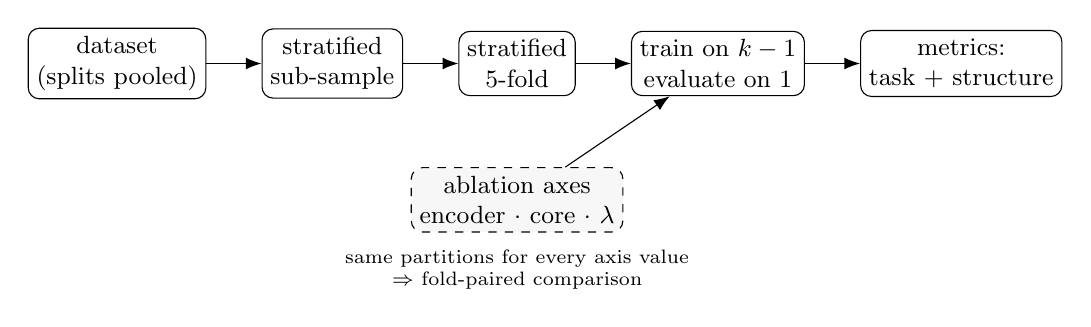
\begin{tikzpicture}[font=\small, node distance=3mm]
\tikzset{
  box/.style={draw, rounded corners, align=center, minimum height=8mm, inner sep=3pt},
  ax/.style={draw, dashed, rounded corners, align=center, inner sep=3pt, fill=black!3},
}
\node[box] (data) {dataset\\(splits pooled)};
\node[box, right=7mm of data] (cap) {stratified\\sub-sample};
\node[box, right=7mm of cap] (fold) {stratified\\5-fold};
\node[ax, below=9mm of fold] (axes) {ablation axes\\encoder $\cdot$ core $\cdot$ $\lambda$};
\node[box, right=7mm of fold] (train) {train on $k-1$\\evaluate on $1$};
\node[box, right=7mm of train] (met) {metrics:\\task $+$ structure};

\draw[-{Latex[length=2mm]}] (data) -- (cap);
\draw[-{Latex[length=2mm]}] (cap) -- (fold);
\draw[-{Latex[length=2mm]}] (fold) -- (train);
\draw[-{Latex[length=2mm]}] (train) -- (met);
\draw[-{Latex[length=2mm]}] (axes) -- (train);
\node[below=1mm of axes, font=\scriptsize, align=center]
  {same partitions for every axis value\\$\Rightarrow$ fold-paired comparison};
\end{tikzpicture}%
}
\caption{The protocol. Fold partitions are fixed by seed and reused across every
configuration of a dataset, which is what makes the comparisons in
Table~\ref{tab:stats} paired rather than independent.}
\label{fig:protocol}
\end{figure}

\subsection{What we measure}

Task performance alone cannot distinguish a network whose groups carry
complementary information from one whose groups are redundant copies, since
both can classify equally well. We therefore report two families.

\textbf{Task.} Accuracy and macro one-vs-rest AUC, which are the metrics the
MedMNIST benchmark~\cite{yang2023medmnist} reports and therefore allow comparison against published
baselines; plus balanced accuracy, macro F1, Cohen's $\kappa$ and MCC. On
imbalanced medical data the gap between accuracy and balanced accuracy is itself
diagnostic: a single class accounts for roughly $67\%$ of DermaMNIST, and a
model that collapses onto it scores well on the former and poorly on the latter.

\textbf{Structure.} Let $z_g$ be the code of group $g$ and $y$ the label.
\begin{itemize}[leftmargin=*, itemsep=1pt, topsep=2pt]
  \item $\mathrm{NMI}(z_g; y)$, averaged over groups, which is how much any
        single group knows on its own;
  \item $\mathrm{NMI}(z_i; z_j)$, averaged over pairs, the \emph{redundancy};
        near zero means independent codes;
  \item \textbf{pair gain}, the quantity the architecture is built to produce:
        \begin{equation}
          \begin{aligned}
            \frac{1}{|E|}\sum_{(i,j)\in E} \Bigl[
              &\mathrm{NMI}\bigl((z_i,z_j); y\bigr)\\
              &- \max_{g \in \{i,j\}} \mathrm{NMI}(z_g;y) \Bigr],
          \end{aligned}
          \label{eq:pairgain}
        \end{equation}
        positive only when a connected pair carries more about the label
        \emph{together} than either member carries alone. This is the
        operational definition of compositionality we commit to;
  \item \textbf{VSA recovery}, the fraction of codes recovered by the
        bundle $\rightarrow$ unbind $\rightarrow$ cleanup round trip of
        Equations~\ref{eq:bundle} and~\ref{eq:cleanup}. It measures whether the
        program remains \emph{readable}, which any downstream composition
        between networks requires;
  \item alphabet utilisation and code perplexity, which detect a collapsed
        bottleneck that classifies well by ignoring most of its vocabulary.
\end{itemize}

\subsection{Reproducibility}

Each run writes its per-fold metrics, the aggregate, the dataset description and
a provenance record (commit hash, working-tree cleanliness, PyTorch version, GPU
model, timestamp) into a single JSON file. The tables and figures in this paper
are generated from those files by \texttt{report.py}, so no number here is
transcribed by hand. The code, the protocol and the result files are in the
project repository.
 depois da seção de trabalhos relacionados.
%
% Requer no preâmbulo (já presentes no template): graphicx, booktabs,
% tikz (arrows.meta, positioning), amsmath.
% =====================================================================

\section{The Sparse-Joint Core}
\label{sec:architecture}

A sparse-joint network replaces the dense bottleneck of a conventional encoder
with a \emph{graded program}: a representation that is simultaneously discrete,
as a tuple of per-group symbols, and continuous, as a hypervector that the
network can differentiate through. This section states the construction
precisely; Section~\ref{sec:protocol} describes how we test it.

\subsection{Groups and the scaffold}

Let $U$ be the number of hidden units per layer, $L$ the number of layers and
$G$ the number of \emph{groups}. A group is a sparse population of units
distributed across layers, fixed before training by a binary mask
$M \in \{0,1\}^{L \times G \times U}$, where $M_{l,g,u}=1$ means that group $g$
owns unit $u$ in layer $l$. We call $M$ the \emph{scaffold}.

Two groups are adjacent when they physically share a unit:
\begin{equation}
  (i,j) \in E \iff \exists\, l,u : M_{l,i,u} = M_{l,j,u} = 1 .
  \label{eq:edges}
\end{equation}
The edge set $E$ is therefore not a hyperparameter chosen alongside the
architecture; it is a \emph{consequence} of the scaffold, readable from the
weights themselves. This is what later allows $E$ to act as a compatibility
certificate between two independently trained networks: two networks with
isomorphic scaffolds expose the same relational skeleton, even though neither
has seen the other's data. Figure~\ref{fig:glue}(a) shows the graph used
throughout this work, for $G=8$.

Unit-to-unit transitions are routed through the scaffold: a connection between
units $u$ and $u'$ exists only if some group contains both. A group therefore
cannot read an arbitrary part of the hidden state, which is what makes the
sparsity structural rather than merely a regulariser.

\subsection{From activations to a program}

Write $h^{(l)} \in \mathbb{R}^{U \times W}$ for the hidden state at layer $l$,
each unit carrying a width-$W$ vector, with
$h^{(0)} = \mathrm{GELU}(W_{\text{in}}\, \phi(x))$ for an encoder $\phi$. Each
group pools the units it owns, across all layers:
\begin{equation}
  f_g = \frac{1}{L}\sum_{l=1}^{L}
        \frac{\sum_{u} M_{l,g,u}\, h^{(l)}_u}{\sum_{u} M_{l,g,u}},
  \qquad
  v_g = \frac{W_{\text{val}} f_g}{\lVert W_{\text{val}} f_g \rVert}.
  \label{eq:pool}
\end{equation}

Each group owns a fixed bipolar \emph{role} vector $r_g \in \{-1,+1\}^{D}$,
drawn once at initialisation. Binding is the Hadamard product, the standard
multiply-add vector-symbolic algebra: $r_g \odot v_g$ binds the group's value to
its identity, and because $r_g \odot r_g = \mathbf{1}$, binding again by the
same role unbinds it. Unary messages are written back to every unit the group
owns, and pairwise messages $r_i v_i \odot r_j v_j$ only to the units that $i$
and $j$ physically share, so interaction is confined to $E$ by construction.
The stack is then re-pooled, giving refined values $v'_g$.

The refined values are superposed into a single hypervector, and each group is
recovered from the superposition by unbinding with its own role:
\begin{equation}
  b = \frac{1}{\sqrt{G}}\sum_{g=1}^{G} r_g \odot v'_g,
  \qquad
  \tilde{v}_g = \sqrt{G}\, \bigl( b \odot r_g \bigr).
  \label{eq:bundle}
\end{equation}
Recovery is approximate: the other $G-1$ terms survive as noise whose magnitude
falls with $D$. We measure this directly (Section~\ref{sec:protocol},
\emph{VSA recovery}) rather than assuming it, because every downstream claim
about reading codes back out depends on it.

\subsection{Discretisation}

Each group owns a codebook $C_g \in \mathbb{R}^{K_g \times D}$ with its own
alphabet size $K_g$, so groups need not share a vocabulary. Cleanup is a cosine
lookup against that codebook,
\begin{equation}
  \ell_{g,c} = \frac{1}{\tau}
  \left\langle \frac{\tilde{v}_g}{\lVert \tilde{v}_g \rVert},
               \frac{C_{g,c}}{\lVert C_{g,c} \rVert} \right\rangle
  + m_{g,c},
  \label{eq:cleanup}
\end{equation}
where $m_{g,c} = -\infty$ for $c \geq K_g$ masks out fillers outside the group's
alphabet. The discrete code is $z_g = \arg\max_c \ell_{g,c}$, and gradients pass
through a straight-through estimator~\cite{bengio2013estimating,oord2017neural}, so the forward pass is exactly discrete
while the backward pass stays differentiable.

The exported \emph{program} is graded, concatenating a unary and a pairwise
bundle:
\begin{equation}
  \begin{aligned}
    P(x) &= \bigl[\, p_{\text{unary}} \;;\; p_{\text{pair}} \,\bigr],\\
    p_{\text{unary}} &= \tfrac{1}{\sqrt{G}}\textstyle\sum\nolimits_g r_g \odot \hat{v}_g,\\
    p_{\text{pair}} &= \tfrac{1}{\sqrt{|E|}}\textstyle\sum\nolimits_{(i,j) \in E}
       \hat{h}_i \odot \hat{h}_j,
  \end{aligned}
  \label{eq:program}
\end{equation}
where $\hat{h}_g = r_g \odot \hat{v}_g$ is the bound contribution of group $g$,
and $\hat{v}_g$ the quantised value of group $g$. The first term says what each
part is; the second says which parts co-occur, and only along scaffold edges.
Figure~\ref{fig:method} traces the whole path.

\subsection{Redundancy between groups}
\label{sec:penalty}

Nothing in Equations~\ref{eq:pool} to~\ref{eq:program} forces groups to encode
\emph{different} things. Trained only to classify, every group independently
converges on the label: the codes become near-copies of one another, and the
pairwise term of Equation~\ref{eq:program} carries nothing the unary term does
not already carry. We confirm this empirically in Section~\ref{sec:results}.

We therefore add a penalty on the mutual information between the soft code
distributions of every pair of groups. Writing $p_g \in \Delta^{K_g}$ for the
posterior of group $g$ on a batch, and $\hat{p}_{ij}$ for the empirical joint,
\begin{equation}
  \mathcal{L}_{\text{red}} =
  \frac{1}{G(G-1)} \sum_{i \neq j}
  \sum_{c,c'} \hat{p}_{ij}(c,c')
  \log \frac{\hat{p}_{ij}(c,c')}{\hat{p}_i(c)\,\hat{p}_j(c')},
  \label{eq:redundancy}
\end{equation}
added to the task loss with weight $\lambda$. Minimising it pushes the groups
towards statistically independent codes. The full objective is
$\mathcal{L} = \mathcal{L}_{\text{task}} + \mathcal{L}_{\text{VQ}}
+ \mathcal{L}_{\text{support}} + \lambda \mathcal{L}_{\text{red}}$.

% =====================================================================

\section{Experimental Protocol}
\label{sec:protocol}

The claims this architecture makes are about generality and about structure,
not only about accuracy, so the protocol has to be comparable across domains
and has to measure structure explicitly.

\subsection{Architecture and ablation axes}

Every result reported here uses the same core configuration: $G=8$ groups,
alphabet $K_g=16$, $U=128$ units, $L=3$ layers, $D=256$, unit width $8$, trained
for 120 epochs with AdamW at a learning rate of $2\times10^{-3}$ and batch
size 1024.\footnote{The epoch count is set so that the number of optimiser steps
matches that of the smaller-batch configuration it replaced, making the two
training budgets comparable.} Only three axes vary, and each is named in the
configuration:

\begin{itemize}[leftmargin=*, itemsep=1pt, topsep=2pt]
  \item \textbf{encoder}, a single dense layer over flattened pixels, or a
        small CNN, both mapping into the same $\phi$ dimensionality;
  \item \textbf{core}, the sparse-joint core or a dense bottleneck of
        identical output dimensionality, used as a control;
  \item \textbf{$\lambda$}, the weight of the redundancy penalty of
        Equation~\ref{eq:redundancy}.
\end{itemize}

This matters for comparability. In an earlier state of this
work the image-classification experiments and the medical-imaging experiments
ran under different core configurations ($L=2, U=32, D=64$ against
$L=3, U=128, D=256$), which makes any cross-domain comparison between them
meaningless. Fixing the architecture is what licenses the generality claim in
Section~\ref{sec:results}.

\subsection{Validation}

We use stratified $k$-fold cross-validation with $k=5$ rather than the official
benchmark splits, pooling all official partitions first. Three consequences
follow, and all three are deliberate:

\begin{enumerate}[leftmargin=*, itemsep=1pt, topsep=2pt]
  \item every sample is evaluated exactly once, which matters on the smaller
        medical datasets where a single test split is noisy;
  \item the fold partitions are generated from a fixed seed and are
        \emph{identical across configurations}, so a comparison between two
        configurations is paired fold by fold;
  \item standardisation statistics are computed on the training fold only.
\end{enumerate}

Datasets are stratified-subsampled to a common ceiling of 17{,}000 samples, so
that MNIST does not receive four times the training budget of BloodMNIST. Where
a comparison is drawn between configurations, we report the paired difference
per fold, Cohen's $d$, and a Wilcoxon signed-rank $p$-value. With five folds
that test has little power; the effect size is the primary reading and the
$p$-value is reported for completeness rather than as a decision rule.

\begin{figure}[!t]
\centering
\resizebox{0.99\linewidth}{!}{%
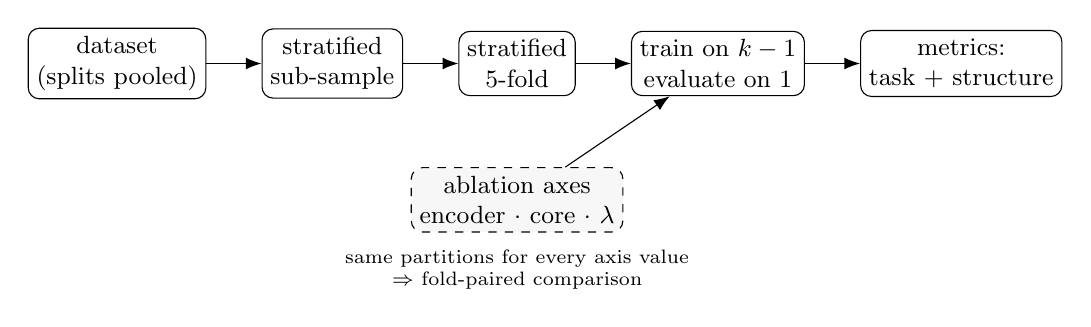
\begin{tikzpicture}[font=\small, node distance=3mm]
\tikzset{
  box/.style={draw, rounded corners, align=center, minimum height=8mm, inner sep=3pt},
  ax/.style={draw, dashed, rounded corners, align=center, inner sep=3pt, fill=black!3},
}
\node[box] (data) {dataset\\(splits pooled)};
\node[box, right=7mm of data] (cap) {stratified\\sub-sample};
\node[box, right=7mm of cap] (fold) {stratified\\5-fold};
\node[ax, below=9mm of fold] (axes) {ablation axes\\encoder $\cdot$ core $\cdot$ $\lambda$};
\node[box, right=7mm of fold] (train) {train on $k-1$\\evaluate on $1$};
\node[box, right=7mm of train] (met) {metrics:\\task $+$ structure};

\draw[-{Latex[length=2mm]}] (data) -- (cap);
\draw[-{Latex[length=2mm]}] (cap) -- (fold);
\draw[-{Latex[length=2mm]}] (fold) -- (train);
\draw[-{Latex[length=2mm]}] (train) -- (met);
\draw[-{Latex[length=2mm]}] (axes) -- (train);
\node[below=1mm of axes, font=\scriptsize, align=center]
  {same partitions for every axis value\\$\Rightarrow$ fold-paired comparison};
\end{tikzpicture}%
}
\caption{The protocol. Fold partitions are fixed by seed and reused across every
configuration of a dataset, which is what makes the comparisons in
Table~\ref{tab:stats} paired rather than independent.}
\label{fig:protocol}
\end{figure}

\subsection{What we measure}

Task performance alone cannot distinguish a network whose groups carry
complementary information from one whose groups are redundant copies, since
both can classify equally well. We therefore report two families.

\textbf{Task.} Accuracy and macro one-vs-rest AUC, which are the metrics the
MedMNIST benchmark~\cite{yang2023medmnist} reports and therefore allow comparison against published
baselines; plus balanced accuracy, macro F1, Cohen's $\kappa$ and MCC. On
imbalanced medical data the gap between accuracy and balanced accuracy is itself
diagnostic: a single class accounts for roughly $67\%$ of DermaMNIST, and a
model that collapses onto it scores well on the former and poorly on the latter.

\textbf{Structure.} Let $z_g$ be the code of group $g$ and $y$ the label.
\begin{itemize}[leftmargin=*, itemsep=1pt, topsep=2pt]
  \item $\mathrm{NMI}(z_g; y)$, averaged over groups, which is how much any
        single group knows on its own;
  \item $\mathrm{NMI}(z_i; z_j)$, averaged over pairs, the \emph{redundancy};
        near zero means independent codes;
  \item \textbf{pair gain}, the quantity the architecture is built to produce:
        \begin{equation}
          \begin{aligned}
            \frac{1}{|E|}\sum_{(i,j)\in E} \Bigl[
              &\mathrm{NMI}\bigl((z_i,z_j); y\bigr)\\
              &- \max_{g \in \{i,j\}} \mathrm{NMI}(z_g;y) \Bigr],
          \end{aligned}
          \label{eq:pairgain}
        \end{equation}
        positive only when a connected pair carries more about the label
        \emph{together} than either member carries alone. This is the
        operational definition of compositionality we commit to;
  \item \textbf{VSA recovery}, the fraction of codes recovered by the
        bundle $\rightarrow$ unbind $\rightarrow$ cleanup round trip of
        Equations~\ref{eq:bundle} and~\ref{eq:cleanup}. It measures whether the
        program remains \emph{readable}, which any downstream composition
        between networks requires;
  \item alphabet utilisation and code perplexity, which detect a collapsed
        bottleneck that classifies well by ignoring most of its vocabulary.
\end{itemize}

\subsection{Reproducibility}

Each run writes its per-fold metrics, the aggregate, the dataset description and
a provenance record (commit hash, working-tree cleanliness, PyTorch version, GPU
model, timestamp) into a single JSON file. The tables and figures in this paper
are generated from those files by \texttt{report.py}, so no number here is
transcribed by hand. The code, the protocol and the result files are in the
project repository.


% =====================================================================
% Seção de resultados.
%
% As tabelas abaixo são GERADAS por report.py a partir dos JSON de
% results/validation/. Não editar os .tex de tabela à mão: rode
%     python validation.py --suite all
%     python report.py
% e copie results/validation/paper/*.tex e *.pdf para junto do artigo.
%
% Números no texto conferidos contra a execução de 2026-10-15,
% commit d57f4d0, PyTorch 2.6.0+cu118, RTX 3060.
% =====================================================================

\section{Results}
\label{sec:results}

Before the individual findings, one property of the design bounds how all of
them may be read. With five folds, the smallest two-sided $p$ a Wilcoxon
signed-rank test can return is $0.062$; no comparison in this section can
therefore reach the conventional $0.05$ threshold, whatever the size of the
underlying effect. This is a property of the sample of folds, not of the
effects, and it is why we report Cohen's $d$ and the number of folds that moved
in each direction as the primary evidence, with $p$ included only for
completeness.

\subsection{Generality across datasets}

Table~\ref{tab:generality} applies the identical core and protocol to four
datasets: two natural-image benchmarks~\cite{lecun1998mnist,xiao2017fashion} and two medical ones
drawn from MedMNIST~v2~\cite{yang2023medmnist}: BloodMNIST, from peripheral blood
smears~\cite{acevedo2020blood}, and DermaMNIST, from dermatoscopic
images~\cite{tschandl2018ham10000}.

\input{table_generality}

A single configuration, chosen once and never retuned per dataset, reaches
$0.986$ accuracy on MNIST, $0.895$ on Fashion-MNIST and $0.937$ on BloodMNIST.
The last of these sits about two points below the published ResNet-18 reference
for the same data at the same resolution, which is a reasonable showing for an
architecture that routes everything through eight discrete symbols on the way
to its decision.

DermaMNIST is the exception. Accuracy reaches $0.726$, close to the
$0.735$ of the ResNet-18 reference, while balanced accuracy is $0.469$ and the
pair gain is slightly \emph{negative} ($-0.010$). The dataset has an imbalance
ratio of $58{:}1$, and the model is substantially predicting the majority class;
accuracy alone would have reported this as a near-baseline success.
Figure~\ref{fig:generality} shows the divergence directly. We keep this case
because it is the reason the protocol reports balanced accuracy and pair gain
alongside accuracy: an evaluation without them would have scored a collapsed
model as a working one.

\begin{figure}[!t]
\centering
\includegraphics[width=0.99\linewidth]{fig_generality.pdf}
\caption{Accuracy and balanced accuracy under the same core and protocol.
Dashed lines mark the published ResNet-18 accuracy for the medical datasets.
The gap between the two bars on DermaMNIST is majority-class collapse: the
dataset is imbalanced $58{:}1$.}
\label{fig:generality}
\end{figure}

\subsection{Encoder and bottleneck}

Table~\ref{tab:encoder} separates two things that are easy to confuse: the
quality of the features entering the core, and the price of the discrete
bottleneck itself. The third variant per dataset removes the core entirely,
keeping the same encoder and the same program dimensionality, so the difference
isolates discretisation.

\input{table_encoder}

The encoder effect is large and consistent. Replacing the dense layer over
flattened pixels with a small CNN moves Fashion-MNIST from $0.858$ to $0.895$
($d=4.94$, 5/5 folds) and BloodMNIST from $0.860$ to $0.937$ ($d=10.68$, 5/5
folds). This is worth stating plainly because an earlier version of these
experiments used the dense encoder throughout and therefore understated the
architecture: what looked like a limitation of the sparse VSA core was mostly a
limitation of what we were feeding it.

The bottleneck effect is smaller. Against the no-core
control, \emph{accuracy is statistically indistinguishable}: the control is
ahead by $0.004$ on Fashion-MNIST ($d=0.61$, 3/5 folds) and behind by $0.002$ on
BloodMNIST ($d=-0.24$, 2/5 folds). Compressing the representation into eight
groups of sixteen symbols costs essentially nothing in decision quality, in
either direction, on either dataset.

The cost appears instead in \emph{ranking}. Macro AUC favours the control
consistently, by $0.008$ on both datasets, with large effect size and all five
folds agreeing in each case ($d=9.05$ and $d=4.99$). The interpretation we
offer is that discretisation preserves the decision boundary while discarding
the graded confidence around it: an argmax over sixteen symbols per group cannot
express the fine differences in certainty that a dense vector carries, and AUC
is the metric that reads those differences. For a downstream use that
needs calibrated scores this matters; for one that needs decisions, it does not.

\subsection{Redundancy penalty}

Trained only to classify, the groups converge on redundant codes: inter-group
NMI sits at $0.54$ on Fashion-MNIST and $0.53$ on BloodMNIST, with pair gains of
only $0.068$ and $0.053$. In that regime the pairwise half of the program adds
little to the unary half. Table~\ref{tab:specialization} and Figure~\ref{fig:tradeoff}
trace what the redundancy penalty of Equation~\ref{eq:redundancy} changes.

\input{table_specialization}

\begin{figure}[!t]
\centering
\includegraphics[width=0.99\linewidth]{fig_tradeoff.pdf}
\caption{Effect of the redundancy penalty. The two datasets track each other
closely in all three panels. Compositionality (left) rises sharply and then
plateaus; redundancy (centre) falls monotonically; readability of the
hypervector (right) degrades and does not recover at larger weights.}
\label{fig:tradeoff}
\end{figure}

\textbf{Effect of the penalty.} At $\lambda=0.25$ the
pair gain more than doubles on both datasets, from $0.068$ to $0.159$ on
Fashion-MNIST ($d=7.87$, 5/5 folds) and from $0.053$ to $0.133$ on BloodMNIST
($d=9.39$, 5/5 folds), while inter-group redundancy halves. Accuracy moves by
$+0.002$ and $-0.003$ respectively, well inside the fold-to-fold spread. The two curves in
Figure~\ref{fig:tradeoff} nearly coincide across a greyscale clothing dataset
and an RGB microscopy dataset, which is the replication evidence available at
this stage.

\textbf{Larger weights.} The pair gain peaks at $\lambda=0.25$ on
both datasets and then flattens or declines, even as redundancy keeps falling
to $0.20$ and $0.18$ at $\lambda=1$. Pushing codes towards independence
eventually removes the shared structure the objective was meant to create:
perfectly independent groups have nothing to compose. The useful range of $\lambda$ is
narrow and at the low end.

\textbf{Effect on readability.} VSA recovery falls from $0.988$ to
$0.872$ on Fashion-MNIST and from $0.991$ to $0.780$ on BloodMNIST at
$\lambda=0.25$, and continues to degrade with larger weights. Code perplexity
falls alongside it, from $6.07$ to $4.39$ and from $4.90$ to $3.66$, which is
consistent with independence being bought by relaxing the separation between
codebook entries, since cleanup (Equation~\ref{eq:cleanup}) is a cosine
lookup against those same entries.

The severity of this cost is sensitive to the training budget, and we report
this because an earlier run misled us. Under a shorter schedule and the dense
encoder, recovery collapsed to roughly $0.65$ at every non-zero weight, which
suggested a hard discontinuity. With the CNN encoder and four times the
optimisation steps, unpenalised recovery rises to $0.99$ and the penalised
value at $\lambda=0.25$ retains $0.87$ on Fashion-MNIST. The conflict between
independence and readability is real and reproducible, but it is a graded
trade-off, not the cliff the earlier evidence implied.

This distinction matters for the architecture's purpose. Composing two
independently trained networks requires reading codes back out of a
superposition; a program that classifies well but decodes poorly is of limited
use for that. At $\lambda=0.25$ the construction buys a doubled pair gain for
roughly twelve points of recovery on Fashion-MNIST and twenty-one on
BloodMNIST, and whether that is a good trade cannot be settled until the
composition step itself is measured.

\subsection{Statistical summary}

Table~\ref{tab:stats} collects the fold-paired comparisons behind the claims
above. Every configuration of a dataset shares its fold partitions, so the
differences are paired by construction.

\input{table_stats}

\subsection{Limitations}

Four limitations bound what the above establishes.

The composition mechanism itself is untested. The routine that \emph{applies} a
Glue, translating codes between algebras, merging with target-private symbols
and composing programs, is implemented and structurally validated,
but the routine that \emph{estimates} the alignment from data is not yet part of
the reproducible pipeline. Every result here therefore concerns a single
network, and the central claim of the project remains open.

The evaluation is confined to $28\times28$ images and to one core
configuration. The generality claim is about domains, not scale: nothing here
shows the construction survives at higher resolution, with more groups, or on
non-visual input.

Five folds give little statistical power, as noted at the outset. The effects we
rely on are large ($d > 4$ throughout), but the design cannot distinguish a
small real effect from none.

Finally, $\lambda$ was held fixed throughout training. A schedule that anneals
it, or an explicit codebook-separation term, might recover the lost readability;
both are untested and are the natural next experiments.


\section{Conclusion}

We set out to validate the representation that a Glue mechanism would have to
operate on, under a protocol strict enough that the answer means something. Four
results follow. A single fixed configuration of the sparse-joint core transfers
across natural and medical images without per-dataset retuning. The discrete
bottleneck is nearly free in accuracy and costs about $0.008$ macro AUC,
locating its price in graded confidence rather than in the decision itself. The
encoder, not the core, was the dominant limitation in our earlier experiments.
And the specialisation that composition depends on does not arise from
supervised training alone: the redundancy penalty of
Equation~\ref{eq:redundancy} roughly doubles the pair gain at $\lambda=0.25$ on
both datasets at no accuracy cost, while degrading hypervector recovery, which
is the very property a Glue needs.

That last tension is the project's open problem and the immediate next step,
alongside bringing the Glue estimation routine into the reproducible pipeline so
that the composition claim itself can be measured rather than argued.


\renewcommand\IEEEbibitemsep{0pt plus .3pt}
\bibliographystyle{IEEEtran}
\bibliography{bibtex}

\end{document}
